\documentclass[10pt,english]{beamer}

\usetheme{default}
\setbeamertemplate{navigation symbols}{\textcolor{blue}{\insertframenumber ~/ \inserttotalframenumber}}

\usepackage{amsmath,amssymb,amsthm}
\usepackage{stmaryrd}
\usepackage{enumerate}
\usepackage{stfloats}
\usepackage{bbm}
\usepackage{pdfpages}
\usepackage{framed}

\usepackage{tikz,pgf,pgfplots}
\usepackage{algorithm,algorithmic}
\usepgflibrary{shapes}
\usetikzlibrary{%
  arrows,%
  arrows.meta,
  shapes.misc,% wg. rounded rectangle
  shapes.arrows,%
  shapes,%
  calc,%
  chains,%
  matrix,%
  positioning,% wg. " of "
  scopes,%
  decorations.pathmorphing,% /pgf/decoration/random steps | erste Graphik
  shadows,%
  backgrounds,%
  fit,%
  petri,%
  quotes
}

\pgfplotsset{compat=1.12}

%\usetheme{Frankfurt}
%\usecolortheme{ldpc}
\useinnertheme{rounded}
\usecolortheme{whale}
\usecolortheme{orchid}


\newcommand{\ul}[1]{\underline{#1}}
\renewcommand{\Pr}{\mathbb{P}}

\newcommand{\getpdfpages}[2]{\begingroup
  \setbeamercolor{background canvas}{bg=}
  \addtocounter{framenumber}{1}
  \includepdf[pages={#1},%
  pagecommand={%
    \expandafter\def\expandafter\insertshorttitle\expandafter{%
      \insertshorttitle\hfill\insertframenumber\,/\,\inserttotalframenumber}}%
  ]{#2}
  \endgroup}

\newcommand{\backupbegin}{
   \newcounter{finalframe}
   \setcounter{finalframe}{\value{framenumber}}
}
\newcommand{\backupend}{
   \setcounter{framenumber}{\value{finalframe}}
}

 \setbeamercolor{bibliography entry author}{fg=black}
 \setbeamercolor{bibliography entry title}{fg=black}
 \setbeamercolor{bibliography entry location}{fg=black}
 \setbeamercolor{bibliography entry note}{fg=black}
 
 \setbeamerfont{bibliography item}{size=\footnotesize}
 \setbeamerfont{bibliography entry author}{size=\footnotesize}
 \setbeamerfont{bibliography entry title}{size=\footnotesize}
 \setbeamerfont{bibliography entry location}{size=\footnotesize}
 \setbeamerfont{bibliography entry note}{size=\footnotesize}
 \setbeamertemplate{bibliography item}{\insertbiblabel}
 
\newlength\tikzwidth
\newlength\tikzheight


\newcommand{\mc}[1]{\mathcal{#1}}
\newcommand{\mbb}[1]{\mathbb{#1}}
\newcommand{\expt}{\mbb{E}}
\newcommand{\dd}{\mathrm{d}}

\def\checkmark{\tikz\fill[scale=0.4](0,.35) -- (.25,0) -- (1,.7) -- (.25,.15) -- cycle;}
\def\greencheck{{\color{green}\checkmark}}
\def\scalecheck{\resizebox{\widthof{\checkmark}*\ratio{\widthof{x}}{\widthof{\normalsize x}}}{!}{\checkmark}}
\def\xmark{\tikz [x=1.4ex,y=1.4ex,line width=.2ex, red] \draw (0,0) -- (1,1) (0,1) -- (1,0);}
\def\redx{{\color{red}\xmark}}

\renewcommand{\footnotesep}{-2pt}

\newif\ifslow
\slowtrue

\begin{document}

\ifslow

\title{ECE 586: Vector Space Methods \\ Chapter 1: Logic, Proofs, and Set Theory}
\author{Henry D. Pfister \\ Duke University}
\date{August 28th, 2019 \\ September 2nd, 2019}
\maketitle

\begin{frame} \frametitle{Introduction}

\begin{itemize}
\item \textcolor{blue}{Statement} (or proposition)

\begin{itemize}
  \setlength\itemsep{1mm}
  \item \textcolor{blue}{An assertion that is true or false, but not both}
  
  \item Ex. ``There are no classes at Duke University today'' \greencheck
  
  \item Ex. ``The real number $\sqrt{2}$ is irrational'' \greencheck
  
  \item Ex. ``Wash your hands before dinner'' \redx

\end{itemize}

\vspace{1mm}

\item Combining statements

\begin{itemize}
  \setlength\itemsep{1mm}
  \item One can also form new statements from old ones using English expressions: and; or; not; if, then; if and only if
  \item Ex. ``Duke is located in Durham, NC \textcolor{red}{or} all real numbers are rational''
  
  \item Note: symbols \textcolor{blue}{$P,Q,R,\ldots$} used to denote abstract statements 

\end{itemize}


\end{itemize}

\end{frame}

\begin{frame} \frametitle{Basic Definitions}

\begin{itemize}

\item Conjunction of $P,Q$ (i.e., $P$ AND $Q$)

\begin{itemize}
  \setlength\itemsep{1mm}
  \item Binary operation on logical propositions (\textcolor{red}{denoted $P \wedge Q$}) that:\\ \hspace{2mm} \textcolor{blue}{is true only if both statements are true, and is false otherwise}
\end{itemize}

\vspace{0.5mm}

\item Disjunction of $P,Q$ (i.e., $P$ OR $Q$)

\begin{itemize}
  \setlength\itemsep{1mm}
  \item Binary operation on logical propositions (\textcolor{red}{denoted $P \vee Q$}) that: \\ \hspace{2mm} \textcolor{blue}{is true if either statement is true, and false otherwise}
\end{itemize}

\vspace{0.5mm}

\item Negation OF $P$ (i.e., NOT $P$)

\begin{itemize}
  \setlength\itemsep{1mm}
  \item Unary operation on a logical proposition (\textcolor{red}{denoted $\neg P$}) that: \\ \hspace{2mm} \textcolor{blue}{is true if the statement is false, and is true otherwise}
\end{itemize}

\vspace{0.5mm}
\item Truth Tables \\
  \begin{center}
  \begin{tabular}{|c|c|c|}
  \hline
  $P$ & $Q$ & $P \wedge Q$ \\
  \hline
  T & T & T \\
  T & F & F \\
  F & T & F \\
  F & F & F \\
  \hline
  \end{tabular}
  \hspace{3mm}
  \begin{tabular}{|c|c|c|}
  \hline
  $P$ & $Q$ & $P \vee Q$ \\
  \hline
  T & T & T \\
  T & F & T \\
  F & T & T \\
  F & F & F \\
  \hline
  \end{tabular}
  \hspace{3mm}
  \begin{tabular}{|c|c|}
  \hline
  $P$ & $\neg P$ \\
  \hline
  T & F \\
  F & T \\
  \hline
  \end{tabular}
  \end{center}
  
  
\end{itemize}

\end{frame}

\begin{frame} \frametitle{Conditional Statements (1)}

\begin{itemize}

\item Conditional Connective \textcolor{red}{$P \rightarrow Q$} (i.e., if $P$, then $Q$)

\begin{itemize}
  \setlength\itemsep{2mm}
  \item Binary operation on logical propositions that:\\ \hspace{2mm} \textcolor{blue}{is false if $P$ is true and $Q$ is false, and is true otherwise} \\

\begin{center}
\begin{tabular}{|c|c|c|}
\hline
$P$ & $Q$ & $P \rightarrow Q$ \\
\hline
T & T & T \\
T & F & F \\
F & T & T \\
F & F & T \\
\hline
\end{tabular}
\end{center}

\item $P$ is called the \textcolor{blue}{antecedent} and $Q$ is called the \textcolor{blue}{consequent}

\end{itemize}
\vspace{1mm}

\item Meaning

\begin{itemize}
\setlength\itemsep{1.5mm}
\item When $P$ is false, some people guess the truth value should be undefined. But, these values are \textcolor{blue}{universally accepted} in logic

\item For motivation, one can think of $P \rightarrow Q$ as a \textcolor{blue}{promise that $Q$ is true whenever $P$ is true}. When $P$ is false, the promise is kept by default

\item Ex. suppose your friend promises \textcolor{blue}{``if it is sunny tomorrow, I will ride my bike"}.  We will say this is \textcolor{blue}{true if they keep their promise}.
If it rains and they don't ride their bike, most people would agree that they have still kept their promise.

\end{itemize}
\end{itemize}

\end{frame}

\begin{frame} \frametitle{Conditional Statements (2)}

\begin{itemize}

\item Biconditional \textcolor{red}{$P \leftrightarrow Q$} (i.e., $P$ if and only if $Q$)

\begin{itemize}
  \setlength\itemsep{1.5mm}
  \item Binary operation on logical propositions that is:\\ \hspace{2mm} \textcolor{blue}{true if $P$ and $Q$ have the same truth value, and false otherwise} \vspace{1mm} \\
   
  \begin{center}
  \begin{tabular}{|c|c|c|}
  \hline
  $P$ & $Q$ & $P \leftrightarrow Q$ \\
  \hline
  T & T & T \\
  T & F & F \\
  F & T & F \\
  F & F & T \\
  \hline
  \end{tabular}
  \end{center} 
  \vspace{1mm}

  \item Identical truth values as: $(P \rightarrow Q) \wedge (Q \rightarrow P)$
  
  \item Ex.``John graduates this term if and only if he passes all his classes''
  
\end{itemize}

\vspace{1mm}

\item Variations on the conditional connective $P \rightarrow Q$

\begin{itemize}
  \setlength\itemsep{2mm}
  \item The \textcolor{blue}{converse} of $P \rightarrow Q$ is the statement $Q \rightarrow P$
  \item The \textcolor{blue}{contrapositive} of $P \rightarrow Q$ is the statement $\neg Q \rightarrow \neg P$
\end{itemize}

\end{itemize}

\end{frame}

  
\begin{frame} \frametitle{Compound Statements}
  

\begin{itemize}
\setlength\itemsep{2mm}
\item It is also useful to consider \textcolor{blue}{compound logical statements} like $$(P \rightarrow R) \wedge (Q \vee \neg R)$$

\item There is also a mechanical way to compute their truth tables: \\
\begin{center}
\begin{tabular}{|c|c|c|ccccccc|}
\hline
$P$ & $Q$ & $R$
& $(P$ & $\rightarrow$ & $R)$ & $\wedge$ & $(Q$ & $\vee$ & $\neg R)$ \\
\hline
T & T & T & T & T & T & T & T & T & F \\
T & T & F & T & F & F & F & T & T & T \\
T & F & T & T & T & T & F & F & F & F \\
T & F & F & T & F & F & F & F & T & T \\
F & T & T & F & T & T & T & T & T & F \\
F & T & F & F & T & F & T & T & T & T \\
F & F & T & F & T & T & F & F & F & F \\
F & F & F & F & T & F & T & F & T & T \\
& & & 1 & 5 & 2 & 7 & 3 & 6 & 4 \\
\hline
\end{tabular} .
\end{center}

\end{itemize}


\end{frame}


\begin{frame} \frametitle{Meta Statements}
  

\begin{itemize}
\setlength\itemsep{2mm}
\item<1-> A meta statement is a logical statement about logical statements


\item<2-> Ex. A \textcolor{blue}{tautology} is a compound statement (e.g., $R(P,Q)$) that \vspace{1mm}
\begin{itemize}
 \setlength\itemsep{1.5mm}
 \item \textcolor{blue}{is true for every valuation of its propositional variables}
 \item Ex. $R(P,Q) = P \vee \neg P \vee Q$ is a tautology
\end{itemize}

\vspace{1mm}

\item<2-> Ex. A \textcolor{blue}{contradiction} is a compound statement (e.g., $R(P,Q)$) that \vspace{1mm}
\begin{itemize}
  \setlength\itemsep{1.5mm}
 \item  \textcolor{blue}{is false for every valuation of its propositional variables}
 \item Ex. $R(P,Q) = P \wedge \neg P \wedge Q$ is a contradiction
\end{itemize}

\vspace{1mm}

\item<3-> An \textcolor{blue}{implication $P \Rightarrow Q$} (for compound statements $P,Q$) \vspace{1mm}
\begin{itemize}
  \setlength\itemsep{1.5mm}
 \item states $Q$ is true whenever $P$ is true (i.e., \textcolor{blue}{$P \rightarrow Q$ is a tautology})
 \item Ex. $(P \rightarrow Q) \wedge P \Rightarrow Q$ holds since $(P \rightarrow Q) \wedge P \rightarrow Q$ is a tautology
\end{itemize}

\item<4-> An \textcolor{blue}{equivalence $P \Leftrightarrow Q$} (for compound statements $P,Q$) \vspace{1mm}
\begin{itemize}
  \setlength\itemsep{1.5mm}
 \item states $P$ is true if and only if $Q$ is true (i.e., \textcolor{blue}{$P \leftrightarrow Q$ is a tautology})
 \item Ex. $P \rightarrow Q \Leftrightarrow \neg P \vee Q$ because $(P \rightarrow Q) \leftrightarrow (\neg P \vee Q)$ is a tautology
\end{itemize}

\end{itemize}


\end{frame}


\begin{frame}{Quantifiers}

\begin{itemize}
\setlength\itemsep{3mm}
\item<1-> The logic we have discussed so far is called \textcolor{blue}{propositional logic}

\item<1-> Limitations of propositional logic \vspace{1mm}
\begin{itemize}
 \setlength\itemsep{1.5mm}
 \item If ``Socrates is a person'' and ``Every person is mortal''
 \item Then, we know ``Socrates is mortal'' but, in propositional logic, there is no way to formally deduce this by combining the statements 
\end{itemize}

\item<2-> \textcolor{blue}{First-order predicate logic} \vspace{1mm}
\begin{itemize}
 \setlength\itemsep{1.5mm}
 \item Let $U$ be a collection of elements and $P(x)$ be a statement that can be applied to any $x\in U$
 \item Ex. $P(x)$ = ``$x$ has 4 tires'' for the collection $U$ of all vehicles
 \item Statement $P(x)$ is called a \textcolor{blue}{predicate} and $x$ is called a \textcolor{blue}{free variable}
\end{itemize}

\item<3-> \textcolor{blue}{Quantifiers}
\begin{itemize}
 \setlength\itemsep{1.5mm}
 \item Quantifiers allow statements about collections of elements
 \item Universal quantifier: $\forall x\!\in\! U, P(x)$ = ``All vehicles have 4 tires''
 \item Existential quantifier: $\exists x\!\in\! U, P(x)$ =``There is a vehicle with 4 tires''
 \item Natural implication: $\forall x \!\in\!U, P(x) \,\Rightarrow\, \exists x\!\in\! U, P(x)$
\end{itemize}



\end{itemize}

\end{frame}

\begin{frame}{Multiple Quantifiers}



\begin{itemize}
\setlength\itemsep{3mm}
\item<1-> Consider predicate $P(x,y)$ with free variables $x,y$ \vspace{1mm}
\begin{itemize}
 \setlength\itemsep{1.5mm}
 \item Ex. Let $I$ be a collection of images and $C$ be a collection of colors. \\ Define predicate $P(x,y)=$``$x$ contains $y$'' for $x\in I$ and $y\in C$ 
 \item ``$\forall x\!\in\! I, \forall y\!\in\! C, P(x,y)$'' = ``All images in $I$ contain all colors in $C$''
 \item ``$\forall x\!\in\! I, \exists y \!\in\! C, P(x,y)$'' = ``All images in $I$ contain some color in $C$''
 \item 8 total possibilities to choose order and quantifiers for each variable
 \item In ``$\exists y \in U, P(x,y)$'', $x$ is a \textcolor{blue}{free variable} and $y$ is a \textcolor{blue}{bound variable}
\end{itemize}

\item<2-> Negation \vspace{1mm}
\begin{itemize}
 \setlength\itemsep{1.5mm}
 \item $\neg (\forall x\!\in\! I, \forall y\!\in\! C, P(x,y))) \,\Leftrightarrow\, \exists x\!\in\! I, \exists y\!\in\! C, \neg P(x,y)$
 \item $\neg (\exists x\!\in\! I, \forall y\!\in\! C, P(x,y)) = \forall x\!\in\! I, \exists y\!\in\! C, \neg P(x,y)$
\end{itemize}  
\item<2-> Natural Implications and Equivalences \vspace{1mm}
%\begin{itemize}
% \setlength\itemsep{1.5mm}
% \item $\forall x\!\in\! I, \forall y\!\in\! C, P(x,y)  \,\Leftrightarrow\, \forall y\!\in\! C, \forall x\!\in\! I, P(x,y)$
% \item $\exists x\!\in\! I, \exists y\!\in\! C, P(x,y) \,\Leftrightarrow\, \exists y\!\in\! C, \exists x\!\in\! I, P(x,y)$
% \item $\forall x\!\in\! I, \forall y\!\in\! C, P(x,y) \,\Rightarrow\, \exists x\!\in\! I, \forall y\!\in\! C, P(x,y)$
% \item Ex. \textcolor{red}{$\exists x\!\in\! I, \forall y\!\in\! C, P(x,y) \,\Rightarrow\, \forall y\!\in\! C, \exists x\!\in\! I, P(x,y)$}   
%\end{itemize}

\vspace{-7mm}
 \item<3->[] {\small \color{blue} \[ \!\!\!\!\!\!\!\!\!\!\!\!\!\!\!\!\!\!\! \begin{array}{ccccccc}
   \forall x, \forall y, P(x,y) & \Rightarrow & \exists x, \forall y, P(x,y) & \Rightarrow & \forall y, \exists x, P(x,y) & \Rightarrow & \exists y, \exists x, P(x,y) \\
   \Updownarrow &&&&&& \Updownarrow \\
   \forall y, \forall x, P(x,y) & \Rightarrow & \exists y, \forall x, P(x,y) & \Rightarrow & \forall x, \exists y, P(x,y) & \Rightarrow & \exists x, \exists y, P(x,y)
   \end{array} \]}

\end{itemize}



%\item<3-> The last implication is more subtle \vspace{1mm}
%\begin{itemize}
%
% \setlength\itemsep{1.5mm}
% \item Ex. $\exists x, \forall y, P(x,y)$ means ``there is an image that contains all the colors'' (e.g., an image of a rainbow)
% \item Ex. $\forall y, \exists x, P(x,y)$ means ``for each color there is an image containing that color''.
% \item The first implies the second because the rainbow image satisfies the $\exists x \forall y$
% \item The implication is not an equivalence, consider a set of pictures where each image contains exactly one color and there is one such image for each color.
%In this case, it is true that ``for each color there is an image containing that color'' but it is not true that `there is an image that contains all the colors''. 
%\end{itemize}
%\end{itemize}

\end{frame}


\begin{frame}{Axiomatic Formulations}

\begin{itemize}
\setlength\itemsep{3mm}
\item<1-> \textcolor{red}{``Ex falso quodlibet''} is Latin for \textcolor{red}{``from falsehood, anything''} \vspace{1mm}
\begin{itemize}
 \setlength\itemsep{1.5mm}
 \item Observe that $P \wedge \neg P \rightarrow Q$ is true regardless of $Q$
 \item Thus, logicians are careful to avoid contradictions
 \item Fortunately, propositional logic has an axiomatic formulation that is consistent, complete, and decidable
\end{itemize} 

\item<2-> What do these words mean in logic? \vspace{1mm}
\begin{itemize} 
 \setlength\itemsep{1.5mm}
 \item \textcolor{blue}{Consistent}: implications of axioms do not contain a contradiction
 \item \textcolor{blue}{Complete}: all valid implications follow from the axioms
 \item \textcolor{blue}{Decidable}: algorithm can determine if any implication is valid or not
\end{itemize}

\item<3-> First-Order Predicate Logic \vspace{1mm}
\begin{itemize} 
 \setlength\itemsep{1.5mm}
 \item Axiomatic formulation is consistent, complete, and semidecidable
 \item \textcolor{blue}{Semidecidable}:  algorithm determines the truth of any postulated implication, if it terminates.  But, termination is guaranteed only if postulate is true
\end{itemize}
\end{itemize}

\end{frame}

\begin{frame}{Strategies for Proofs}

\begin{itemize}
\setlength\itemsep{3mm}
\item<1-> Background
\begin{itemize} 
 \setlength\itemsep{1.5mm}
 \item Intuition identifies what might be true and why
 \item Rigorous proofs verify and communicate that intuition
 \item A \textcolor{blue}{proof} is a sequence of verifiable steps from premises to the result
 \item Definitions act as equivalences between words and symbols 
\end{itemize}

\item<2-> Types of Proofs for $P \rightarrow Q$
\begin{itemize} 
 \setlength\itemsep{1.5mm}
 \item \textcolor{blue}{Direct}: Assume $P$ true and give steps that lead to $Q$
 \item \textcolor{blue}{Contrapositive}: Proof of equivalent statement $\neg Q \rightarrow \neg P$
 \item \textcolor{blue}{Contradiction}: Using $\neg (P \rightarrow Q) \Leftrightarrow P \wedge \neg Q$, one supposes that both $P$ and $\neg Q$ are true and then gives steps leading to a contradiction
 \item \textcolor{blue}{Induction}: For predicate $P(n)$, prove $Q=$``$\forall n\in\mathbb{N}, P(n)$'' by establishing the premise $P=$``$P(1) \wedge (\forall n\in \mathbb{N}, P(n) \rightarrow P(n\!+\!1))$''
\end{itemize}

\item<3-> Whiteboard Examples \vspace{1mm}
\begin{itemize} 
 \setlength\itemsep{1.5mm}
 \item Prove $\sqrt{2}$ is irrational by showing contrapositive via contradiction
 \item For $P(n)=$``$\sum_{i=1}^n i = \frac{n^2 + n}{2}$'', prove ``$\forall n\in \mathbb{N}, P(n)$'' via induction
\end{itemize}
\end{itemize}

\end{frame} 

\begin{frame}{Set Theory}

\begin{itemize}
\setlength\itemsep{3mm}
\item<1-> Foundation (along with logic) of all modern mathematics \vspace{1mm}
\begin{itemize} 
  \setlength\itemsep{1.5mm}
  \item Numbers, relations, functions, \ldots all defined using set theory
  \item Not as easy as it seems because simple approaches include paradoxes (i.e., statements which are both true and false)
  \item Axiomatic framework resolves paradoxes but not useful for engineers
  \item We adopt \textcolor{blue}{naive set theory}, which defines the operations of set theory without worrying about paradoxes. It is sufficient for most math.
\end{itemize}

\item<2-> Naive Set Theory \vspace{1mm}
\begin{itemize} 
  \setlength\itemsep{1.5mm}
  \item \textcolor{blue}{Set defined as ``any collection of objects, mathematical or otherwise''}
  \item Ex. Consider ``the set of all books published in 2007''
  \item Objects in a set are called \textcolor{blue}{elements} or \textcolor{blue}{members} of the set
  \item Logical statement: ``$a$ is a member of the set $A$'' is written \textcolor{blue}{$a \in A$}
  \item Its negation: ``$a$ is not a member of the set $A$'' is written \textcolor{blue}{$a \notin A$}
\end{itemize}
\end{itemize}
\end{frame}

\begin{frame}{Using Set Theory}

\begin{itemize}
\setlength\itemsep{3mm}
\item<1-> Defining Sets \vspace{1mm}
\begin{itemize} 
  \setlength\itemsep{1.5mm}
  \item One can present a set by listing elements: standard English vowels \[A= \{ a,e,i,o,u \} \]
  \item Element order is irrelevant: $\{ i,o,u,a,e \}$ is the same as $A$
  \item Repeated elements have no effect: $\{ a,e,i,o,u,e,o \}$ same as $A$
  \item \textcolor{blue}{Singleton} is a set containing exactly one element such as $\{a\}$
  \item Standard sets: Integers $\mathbb{Z}$, Real numbers $\mathbb{R}$, and Complex numbers $\mathbb{C}$
  %\item It is possible to construct each of these sets in a rigorous manner. Instead, we assume their meaning is intuitively clear
\end{itemize}

\item<2-> Building new sets from old \vspace{1mm}
\begin{itemize} 
  \setlength\itemsep{1.5mm}
  \item \textcolor{blue}{Set-builder notation}: For logical predicate $P(x)$ defined on $x\in X$, ``$A$ is the set of elements in $X$ such that $P(x)$ is true'' is denoted by
\[ A = \{ x\in X | P(x) \} \]
  \item If no $x\in X$ satisfies $P(x)$, then result is an \textcolor{blue}{empty set}, denoted by $\emptyset$
  \item Ex. natural numbers $\mathbb{N}$ and positive prime integers $P$:
\begin{align*}
  \mathbb{N} &= \{ x\in \mathbb{Z} | x\geq 1 \} = \{ 1,2,3,4,\ldots \} \\
  P &= \{ x\in \mathbb{Z} | x\geq 1 \textrm{ and ``}x\textrm{ is prime''} \} = \{ 2,3,5,7,11,\ldots \}
\end{align*}
\end{itemize}
\end{itemize}
\end{frame}

\iffalse
\begin{frame}{Intervals?}

\begin{itemize}
\setlength\itemsep{3mm}
\item<1-> Defining Sets \vspace{1mm}
\begin{itemize} 
  \setlength\itemsep{1.5mm}


\end{itemize}
\end{itemize}
\end{frame}
\fi

\begin{frame}{Set Properties}

\begin{itemize}
\setlength\itemsep{3mm}
%\item<1-> Standard notation for real-interval subsets:
%\begin{align*}
%\textrm{Open interval:} \; &  (a,b) \triangleq \{ x\in \mathbb{R} | a<x<b \} \\
%\textrm{Closed interval:} \; & [a,b] \;\;\!\! \triangleq \{ x\in \mathbb{R} | a \leq x \leq b \} \\
%\textrm{Half-open intervals:} \; & (a,b] \;\! \triangleq \{ x\in \mathbb{R} | a < x \leq b \} \\
%& [a,b) \;\! \triangleq \{ x\in \mathbb{R} | a \leq x < b \}
%\end{align*}

\item<1-> Cardinality \vspace{1mm}
\begin{itemize} 
  \setlength\itemsep{1.5mm}
  \item For set $A$, the \textcolor{blue}{cardinality} $|A|$ is the number of elements in $A$
  \[ |\{ a,e,i,o,u \}| = 5 \]
  \item If there is a one-to-one correspondence between $A$ and the natural numbers $\mathbb{N}$, then $A$ is called \textcolor{blue}{countably infinite} and  $|A| = \infty$
  \item Ex. Set of \textcolor{blue}{rational numbers $\mathbb{Q} \triangleq \{ q \in \mathbb{R} \,|\, \exists n \in \mathbb{N}, nq \in \mathbb{Z} \}$} is countably infinite (e.g., list rationals $m/n$ with $|m|\leq n^2$)
  \item If $|A| = \infty$ but not countably infinite, then $A$ is \textcolor{blue}{uncountably infinite}
  \item Ex. The set of real numbers is uncountably infinite by Cantor's diagonal argument
  
\end{itemize}
\end{itemize}
\end{frame}

% Definition of circles
\def\firstcircle{(0,0) circle (1.5cm)}
\def\secondcircle{(0:2cm) circle (1.5cm)}

\colorlet{circle edge}{blue!50}
\colorlet{circle area}{blue!20}

\tikzset{filled/.style={fill=circle area, draw=circle edge, thick},outline/.style={draw=circle edge, thick}}

\setlength{\parskip}{5mm}

\begin{frame}{Venn Diagrams*}

% Sets A , B
\begin{tikzpicture}
    \draw[outline] \firstcircle node {$A$};
    \draw[outline] \secondcircle node {$B$};
    %\node[anchor=south] at (current bounding box.north) {$A \cap B$};
\end{tikzpicture}
\hfill
% Set A and B
\begin{tikzpicture}
    \begin{scope}
        \clip \firstcircle;
        \fill[filled] \secondcircle;
    \end{scope}
    \draw[outline] \firstcircle node {$A$};
    \draw[outline] \secondcircle node {$B$};
    \node[anchor=south] at (current bounding box.north) {$A \cap B$};
\end{tikzpicture}

% Set A or B
\begin{tikzpicture}
    \draw[filled] \firstcircle node {$A$}
                  \secondcircle node {$B$};
    \node[anchor=south] at (current bounding box.north) {$A \cup B$};
\end{tikzpicture}
\hfill
% Set A but not B
\begin{tikzpicture}
    \begin{scope}
        \clip \firstcircle;
        \draw[filled, even odd rule] \firstcircle node {$A$}
                                     \secondcircle;
    \end{scope}
    \draw[outline] \firstcircle
                   \secondcircle node {$B$};
    \node[anchor=south] at (current bounding box.north) {$A - B$};
\end{tikzpicture}
    
\end{frame}

\begin{frame}{Relationships and Operations Between Sets*}

\begin{itemize}
\setlength\itemsep{3mm}
\item<1-> Operations on sets $A,B$ \vspace{1mm}
\begin{itemize} 
  \setlength\itemsep{1.5mm}
  \item \textcolor{blue}{Union} of $A$ and $B$ ($A\cup B$): set of elements in either $A$ or $B$
%This means that $A \cup B = \{ x\in A \textrm{ or } x\in B \}$ is also defined by
\[ x\in A\cup B \Leftrightarrow (x\in A)\vee (x\in B) \]
  \item \textcolor{blue}{Intersection} of $A$ and $B$ ($A\cap B$): set of elements in both $A$ and $B$
%This means that $A\cap B = \{x\in A | x\in B \}$ is also defined by
\[ x\in A\cap B \Leftrightarrow (x\in A)\wedge (x\in B) \]
  \item \textcolor{blue}{Set difference} $A-B$ (or $A \setminus \!B$): set of elements in $A$ but not in $B$
%This means that
\[ x\in A-B \Leftrightarrow (x\in A)\wedge (x\notin B) \]
  \item \textcolor{blue}{Complement} ($A^c$) for implied universal set $U$  defined by $A^c = U-A$
\end{itemize}

\item<2-> Relationships between sets $A,B$ \vspace{1mm}
\begin{itemize} 
  \setlength\itemsep{1.5mm}
  \item $A$ \textcolor{blue}{equals} $B$ (denoted $A=B$) if both sets have the same elements
\[ ``A=B" \Leftrightarrow \forall x \left( (x\in A)\leftrightarrow (x\in B) \right) \]
  \item $A$ is a \textcolor{blue}{subset} of $B$ (denoted $A\subseteq B$) if all elements in $A$ are also in $B$
\[ ``A\subseteq B"  \Leftrightarrow \forall x \left( (x\in A)\rightarrow (x\in B) \right) \]
  \item $A$ is a \textcolor{blue}{proper subset} of $B$ (denoted $A\subset B$) if $A\subseteq B$ and $A\neq B$
  \item Two sets are \textcolor{blue}{disjoint} if $A\cap B = \emptyset$
\end{itemize}

\end{itemize}
\end{frame}


\begin{frame}{De Morgan, Infinite Unions, and Tuples}

\begin{itemize}
\setlength\itemsep{3mm}
\item<1-> De Morgan's logical identity $\neg (P \vee Q) = \neg P \wedge \neg Q$ for sets:
\begin{align*}
(A \cup B)^c & = A^c \cap B^c \\
(A \cap B)^c & = A^c \cup B^c,
\end{align*}

\item<2-> Also holds for infinite unions and intersections:
  \begin{align*}
  \bigcup_{\alpha \in I} S_{\alpha}
  &\triangleq \{ x | x \in S_{\alpha} \text{ for some } \alpha \in I \} \\
  \bigcap_{\alpha \in I} S_{\alpha}
  &\triangleq \{ x | x \in S_{\alpha} \text{ for all } \alpha \in I \} 
  \end{align*}  

\item<3-> Sets of tuples and vectors \vspace{1mm}
\begin{itemize}
  \setlength\itemsep{1.5mm}
  %Build sets by grouping elements into vectors
  \item For sets $A,B$, the \textcolor{blue}{Cartesian product} $A\times B$ is the set of ordered pairs \[\{(a,b) | a\in A, b\in B\}\]
  \item For $n$-tuples from the same set, we have $A^n=A\times A \times \cdots \times A$
  \item Ex. The set of all 3-tuples from with elements in $A  = \{ a,b \}$ is
\begin{equation*}
\!\!\!\!\!\!\!\!\!\!\!\!\!\!\!\!\!\!\! A^3 = \{ (a,a,a),(a,a,b),(a,b,a),(a,b,b),(b,a,a),(b,a,b),(b,b,a),(b,b,b) \}
\end{equation*}
\end{itemize}
  
\end{itemize}
\end{frame}

\begin{frame}{Foundations of Set Theory}

\begin{example}[Russell's Paradox]
Let $R = \{S|S\notin S\}$ be the set of all sets that do not contain themselves.
This set exists in naive set theory (though it may empty) because it is described by the above sentence.
The paradox arises from the fact that this definition leads to the logical contradiction: $R\notin R \leftrightarrow R\in R$.
\end{example}

\vspace{5mm}

\begin{itemize}
\setlength\itemsep{3mm}
\item<1-> What does this mean? \vspace{1mm}
\begin{itemize} 
  \setlength\itemsep{1.5mm}
  \item This shows that \textcolor{blue}{naive set theory is not consistent} because it allows constructions leading to contradictions
  \item Issue avoided in axiomatic formulation by restricting constructions
  \item Also implies that $R$ cannot exist in any consistent set theory
  %\item Are their sets that contains themselves? In naive set theory, the answer is yes.  Some examples are the ``set of all sets'' and the ``set of all abstract ideas''
  %\item ZF axiomatic formulation has theorem: ``no set contains itself''
\end{itemize}

\end{itemize}
\end{frame}


\begin{frame}{Abstract Relations}

\vspace{3mm}
\begin{definition}
A \textcolor{blue}{relation} $\sim$ between elements of $A$ is defined by the subset $E \subseteq A\times A$.  Specifically, the relation $a \sim b$ holds if and only if $(x,y)\in E$.
\end{definition}
\vspace{-5mm}

\begin{itemize}
\setlength\itemsep{3mm}
\item<1-> Properties: A relation on $A$ is said to be: \vspace{1mm}
\begin{itemize}
  \setlength\itemsep{1.5mm}
  \item \textcolor{blue}{Reflexive} if $x\sim x$ holds for all $x\in A$
  \item \textcolor{blue}{Symmetric} if $x\sim y$ implies $y\sim x$ for all $x,y\in A$
  \item \textcolor{blue}{Transitive} if $x\sim y$ and $y\sim z$, then $x\sim z$ for all $x,y,z\in A$
\end{itemize}

\item<2-> Called an \textcolor{blue}{equivalence relation} if reflexive, symmetric, and transitive \vspace{1mm}

\begin{itemize}
  \setlength\itemsep{1.5mm}
  %\item Abstract generalization of equality
  \item Ex. let $A$ be a set of people and $P(x,y)$ be the statement: \\ \textcolor{blue}{``$x$ has the same birthday (month and day) as $y$''}
  \item Define \textcolor{blue}{relation $\sim$} such that \textcolor{blue}{$a\sim b$} holds iff $P(x,y)$ is true
  %\item For this, $E = \{ (x,y)\in A\times A | P(x,y) \}$
  \item Partitions $A$ into disjoint \textcolor{blue}{equivalence classes}: $[a] \triangleq \left\{x\in A | x \sim a\right\}$
  \item This example has an equivalence class for each possible day in a year
  \item Set of equivalence classes called the \textcolor{blue}{quotient set}: $A \setminus \!\sim \;\triangleq \{ [a] | a\in A \}$

\end{itemize}
\end{itemize}
\end{frame}

\begin{frame}{Functions}

\vspace{3mm}

\begin{definition}
A \textcolor{blue}{function} $f \colon X \rightarrow Y$ from $X$ to $Y$ is defined by a subset $F \subset X \times Y$ such that $A_x = \{ y\in Y | (x,y)\in F \}$ has exactly one element for each $x\in X$.
The \textcolor{blue}{value} of $f$ at $x\in X$, \textcolor{blue}{denoted $f(x)$}, is unique element in $A_x$.
\end{definition}
\vspace{-4mm}

\begin{itemize}
\setlength\itemsep{3mm}
\item<1-> Unpacking the definition \vspace{1mm}
\begin{itemize} 
  \setlength\itemsep{1.5mm}
  \item Function $f \colon X\rightarrow Y$ assigns one value $f(x)\in Y$ to each $x\in X$
  \item Notation \textcolor{blue}{$f \colon X \rightarrow Y$} emphasizes the \textcolor{blue}{domain} $X$ and the \textcolor{blue}{codomain} $Y$
  \item \textcolor{blue}{Range} of $f$ is subset of $Y$ achieved by $f$, $\{y \in Y | \exists x\in X, y=f(x) \}$
  \item Since term codomain is uncommon, people sometimes use the term range instead of codomain either intentionally or unintentionally
\end{itemize}

\item<2-> In basic math, functions are described by graphs and formulas \vspace{1mm}
\begin{itemize} 
  \setlength\itemsep{1.5mm}
  \item This leads students to picture only ``nice'' functions
  \item Ex. Cauchy published \textcolor{blue}{incorrect proof of false assertion}: ``sequence of continuous functions converging everywhere has a continuous limit''
  \item Teachers now warn: \textcolor{blue}{the world is filled with ``not so nice'' functions}
\end{itemize}

\end{itemize}
\end{frame}  

\begin{frame}{Properties of Functions}

\begin{itemize}
\setlength\itemsep{3mm}
\item<1-> Equality \vspace{1mm}
\begin{itemize}
  \setlength\itemsep{1.5mm}
  \item Two functions are \textcolor{blue}{equal} if they have the same domain, codomain, and value for all elements of the domain
\end{itemize}

\item<2-> A function $f$ is called: \vspace{1mm}
\begin{itemize}
  \setlength\itemsep{1.5mm}
  \item \textcolor{blue}{one-to-one} or \textcolor{blue}{injective} if, $\forall x,x'\in X$, if $f(x)=f(x')$ then $x=x'$
  \item \textcolor{blue}{onto} or \textcolor{blue}{surjective} if its range $\{ f(x) | x\in X\}$ equals $Y$
  \item \textcolor{blue}{one-to-one correspondence} or \textcolor{blue}{bijective} if both one-to-one and onto
\end{itemize}

\item<3-> Inversion \vspace{1mm}
\begin{itemize}
  \setlength\itemsep{1.5mm}
  \item A bijective function has a unique \textcolor{blue}{inverse function} $f^{-1} \colon Y\rightarrow X$ satisfying: $\forall x\in X, f^{-1}(f(x)) = x$ and $\forall y\in Y, f(f^{-1}(y)) = y$
  \item Any one-to-one function $f \colon X\rightarrow Y$ defines a bijective function $g \colon X \rightarrow R$ with $g(x)=f(x)$ by choosing range $R$ to be codomain

\end{itemize}

\end{itemize}
\end{frame}    

\begin{frame}{Applying Functions to Sets}

\vspace{4mm}
\begin{definition}
For $f \colon X\rightarrow Y$ and subset $A\subseteq X$, the \textcolor{blue}{image} of $A$ under $f$ is \vspace{-2mm}
\[ f(A) \triangleq \{ y\in Y | \exists x\in A \textrm{ s.t. } f(x)=y\} = \{f(x) | x\in A\}. \]
\end{definition}
\vspace{0mm}
\begin{definition}
The \textcolor{blue}{inverse image} or \textcolor{blue}{preimage} of a subset $B\subseteq Y$ is \vspace{-2mm}
\[ f^{-1}(B) \triangleq \{ x\in X | f(x)\in B\}. \]
\end{definition}
\vspace{-4.5mm}

\begin{itemize}
\setlength\itemsep{3mm}
\item<2-> Properties \vspace{1mm}
\begin{itemize}
  \setlength\itemsep{1.5mm}
  \item This implies that the range of $f$ is simply $f(X)$
  \item Allowing set-valued images means \textcolor{blue}{set-valued inverse always exists}
  \item For a one-to-one $f$, inverse image of singleton $\{ f(x) \}$ is singleton $\{ x \}$
  \item In general, one can show: $f(f^{-1}(B)) \subseteq B$ and $f^{-1}(f(A)) \supseteq A$.
  \item<3-> Ex. For $f \colon \mathbb{R} \rightarrow \mathbb{R}$ defined by $f(x)=x^2$, let $A=[1,2]$ and notice that $B = f(A) = [1,4]$.  But, $f^{-1}(B) = [-2,-1] \cup [1,2] \supseteq A$
  \item<4-> Ex. For $f \colon \mathbb{R} \rightarrow \mathbb{R}$ defined by $f(x)=x^2+1$, let $B=[0,2]$ and notice that $A = f^{-1}(B) = [-1,1]$.  But, $f(A) = f([-1,1]) = [1,2] \subseteq B$
\end{itemize}
\end{itemize}

\end{frame}  
  
%\begin{frame}{Quantifiers}
%
%\vspace{3mm}
%\hspace*{55mm}
%\input{myfigs/mlp2}
%\vspace{-22mm}
%
%\begin{itemize}
%\item<1-> Neural network
%
%\begin{itemize}
%	\item function $f_\theta$ from $\mathcal{X}=\mathbb{R}^n$ to $\mathcal{Y} = \mathbb{R}^d$ \vspace{1mm}
%	%\item \textcolor{snowymint}{function $f_\theta$} from \textcolor{sail}{$\mathcal{X}=\mathbb{R}^n$} to \textcolor{}{$\mathcal{Y} = \mathbb{R}^d$} \vspace{1mm}
%	%\item $z^{\ell+1} = \sigma ( W_{\ell} z^{\ell} )$
%	\item weights represented by $\theta \in \mathbb{R}^p$ \vspace{1mm}
%\end{itemize}
%
%\vspace{1mm}
%
%\item<2-> Training set  
%
%\begin{itemize}
%	\item Set of tuples $(x,y) \in \mathcal{X} \times \mathcal{Y}$ \vspace{1mm}
%	\item For classification into $d$ classes, let $y\in \mathcal{Y}$ be a one-hot vector \vspace{1mm}
%	\item Entire training set denoted $\mathcal{D} \subset \mathcal{X} \times \mathcal{Y}$ \vspace{1mm}
%\end{itemize}
%
%\only<3->{\vspace{-2.5mm}
%\hspace*{62mm}
%%\includegraphics[width=1.75in]{webfigs/vgg56noshort.png}
%\vspace{-36mm}}
%
%\item<3-> Loss function  
%
%\begin{itemize}
%\vspace{1mm}
%	\item Cross entropy: $L (y,\hat{y}) \triangleq - \sum_{i=1}^d y_i \ln \hat{y}_i$ \vspace{1mm}
%	\item Loss for entire training set is
%	\\[-2mm] \[ \hspace*{-32mm} \mathcal{L}_{\mathcal{D}} (\theta) \triangleq \frac{1}{|\mathcal{D}|}\sum_{(x,y) \in \mathcal{D}} L (y,f_\theta (x)) \]
%	\item note: assume $f_\theta (x) \in \mathbb{R}^d$ non-negative and sums to 1 
%\end{itemize}
%
%
%\end{itemize}
%
%\let\thefootnote\relax\footnotetext{\hspace*{-4mm}  {\tiny Loss landscape taken from \url{https://www.cs.umd.edu/~tomg/img/landscapes/noshort.png} \cite{Li-nips18}}}
%
%\end{frame}
%
%\begin{frame}{Neural Network Training}
%
%\vspace{4mm}
%
%\hspace*{62mm}
%%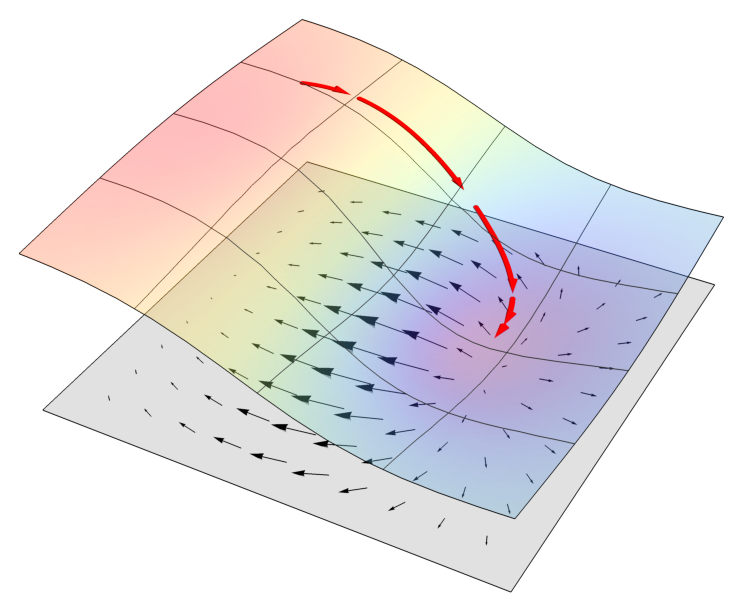
\includegraphics[width=2in]{myfigs/gradient.pdf}
%\vspace{-46mm}
%
%\begin{itemize}
%
%\item<1-> Loss $\mathcal{L}_\mathcal{D} (\theta)$ \textcolor{blue}{landscape} 
%
%\begin{itemize}
%    \item Adjust $\theta \in \mathbb{R}^p$ to minimize loss \vspace{1mm} 
%    \item Gradient vector $\nabla \mathcal{L}_\mathcal{D} (\theta)$ gives \\ $\theta$ direction of maximum increase \vspace{1mm}
%
%\end{itemize}
%
%\vspace{2mm}
%
%%\only<2->{\hspace*{65mm}
%%\includegraphics[width=2.0in]{webfigs/gradient_descent.jpg}
%%\vspace{-34mm}}
%
%\item<2-> Gradient descent (GD) and SGD
%
%\begin{itemize}
%	%\item Full differential: $\frac{d}{dt} \theta_t = - \nabla \mathcal{L} (\theta_t )$  \vspace{1mm}
%	\item full-batch: $\theta_{t + 1} = \theta_t-\eta \, \nabla \mathcal{L}_\mathcal{D} (\theta_t )$  \vspace{1mm}
%	\item \textcolor{blue}{mini-batch}: subset $\mathcal{S}_t \! \subset \! \mathcal{D}$ with $|\mathcal{S}_t|=m$ \\[-2mm] \[ \hspace*{-35mm} \theta_{t + 1} = \theta_t-\eta \, \nabla \mathcal{L}_{\mathcal{S}_t} (\theta_t ) \]  \vspace{1mm}
%\end{itemize}
%
%\vspace{-5.5mm}
%
%\item<3-> Generalization
%
%\begin{itemize}
%	\item The test set $\mathcal{T} \subset \mathcal{X} \times \mathcal{Y}$ contains held-out training data \vspace{1mm}
%	
%	\item Actual goal is to \textcolor{red}{minimize $\mathcal{L}_\mathcal{T}(\theta)$ without knowing $\mathcal{T}$!} \vspace{1mm}
%	
%\end{itemize}
%
%\end{itemize}
%
%%\let\thefootnote\relax\footnotetext{\hspace*{-4mm} {\tiny Figure: \url{https://reconsider.news/2018/05/09/ai-researchers-allege-machine-learning-alchemy/}} }
%
%\end{frame}



\backupbegin

%\begin{frame}
%\frametitle{Backup Slides}
%\begin{itemize}
%\item Slide numbers not included in denominator!
%\end{itemize}
%\end{frame}

%\begin{frame}[allowframebreaks]
%\frametitle{References}
%\bibliographystyle{alpha}
%\footnotesize
%\bibliography{IEEEabrv,WCLabrv,WCLbib,WCLnewbib}
%\end{frame}

\backupend

\end{document}
